\section{Experimental Results}

{\color{red} Things to answer.}
\begin{itemize}
\item Are different algorithms affected differently by frequency adjustment?
\item How does frequency affect performance/energy/power?
\item End with SCI cluster and Titan results, and extrapolate from prior 
measurements.
\end{itemize}


\begin{table*}[tb]
  \begin{center}
  %\resizebox{0.95\textwidth}{!}{
  \begin{tabular}{| l | r | r | r | r | r | r | r |}
  \hline
  \textbf{Variant} & \textbf{Performance} & $\mathbf{\frac{Throughput}{Energy}}$ & $\mathbf{\frac{Throughput}{(Energy)^2}}$ & $\mathbf{\frac{(Throughput)^2}{Energy}}$ & $\mathbf{\frac{Throughput}{Power}}$ & $\mathbf{\frac{Throughput}{(Power)^2}}$ & $\mathbf{\frac{(Throughput)^2}{Power}}$ \\ \hline
  \textbf{Merge Sort} & 0 & 0 & 0 & 0 & 0 & 0 & 0 \\ \hline
  \textbf{Radix Sort} & 0 & 0 & 0 & 0 & 0 & 0 & 0 \\ \hline
  \end{tabular}
  %}
  \end{center}
  \caption{Distribution of variant selections across inputs}
  \label{tab:ss}
\end{table*}

\begin{figure*}[tb]
   \centering
   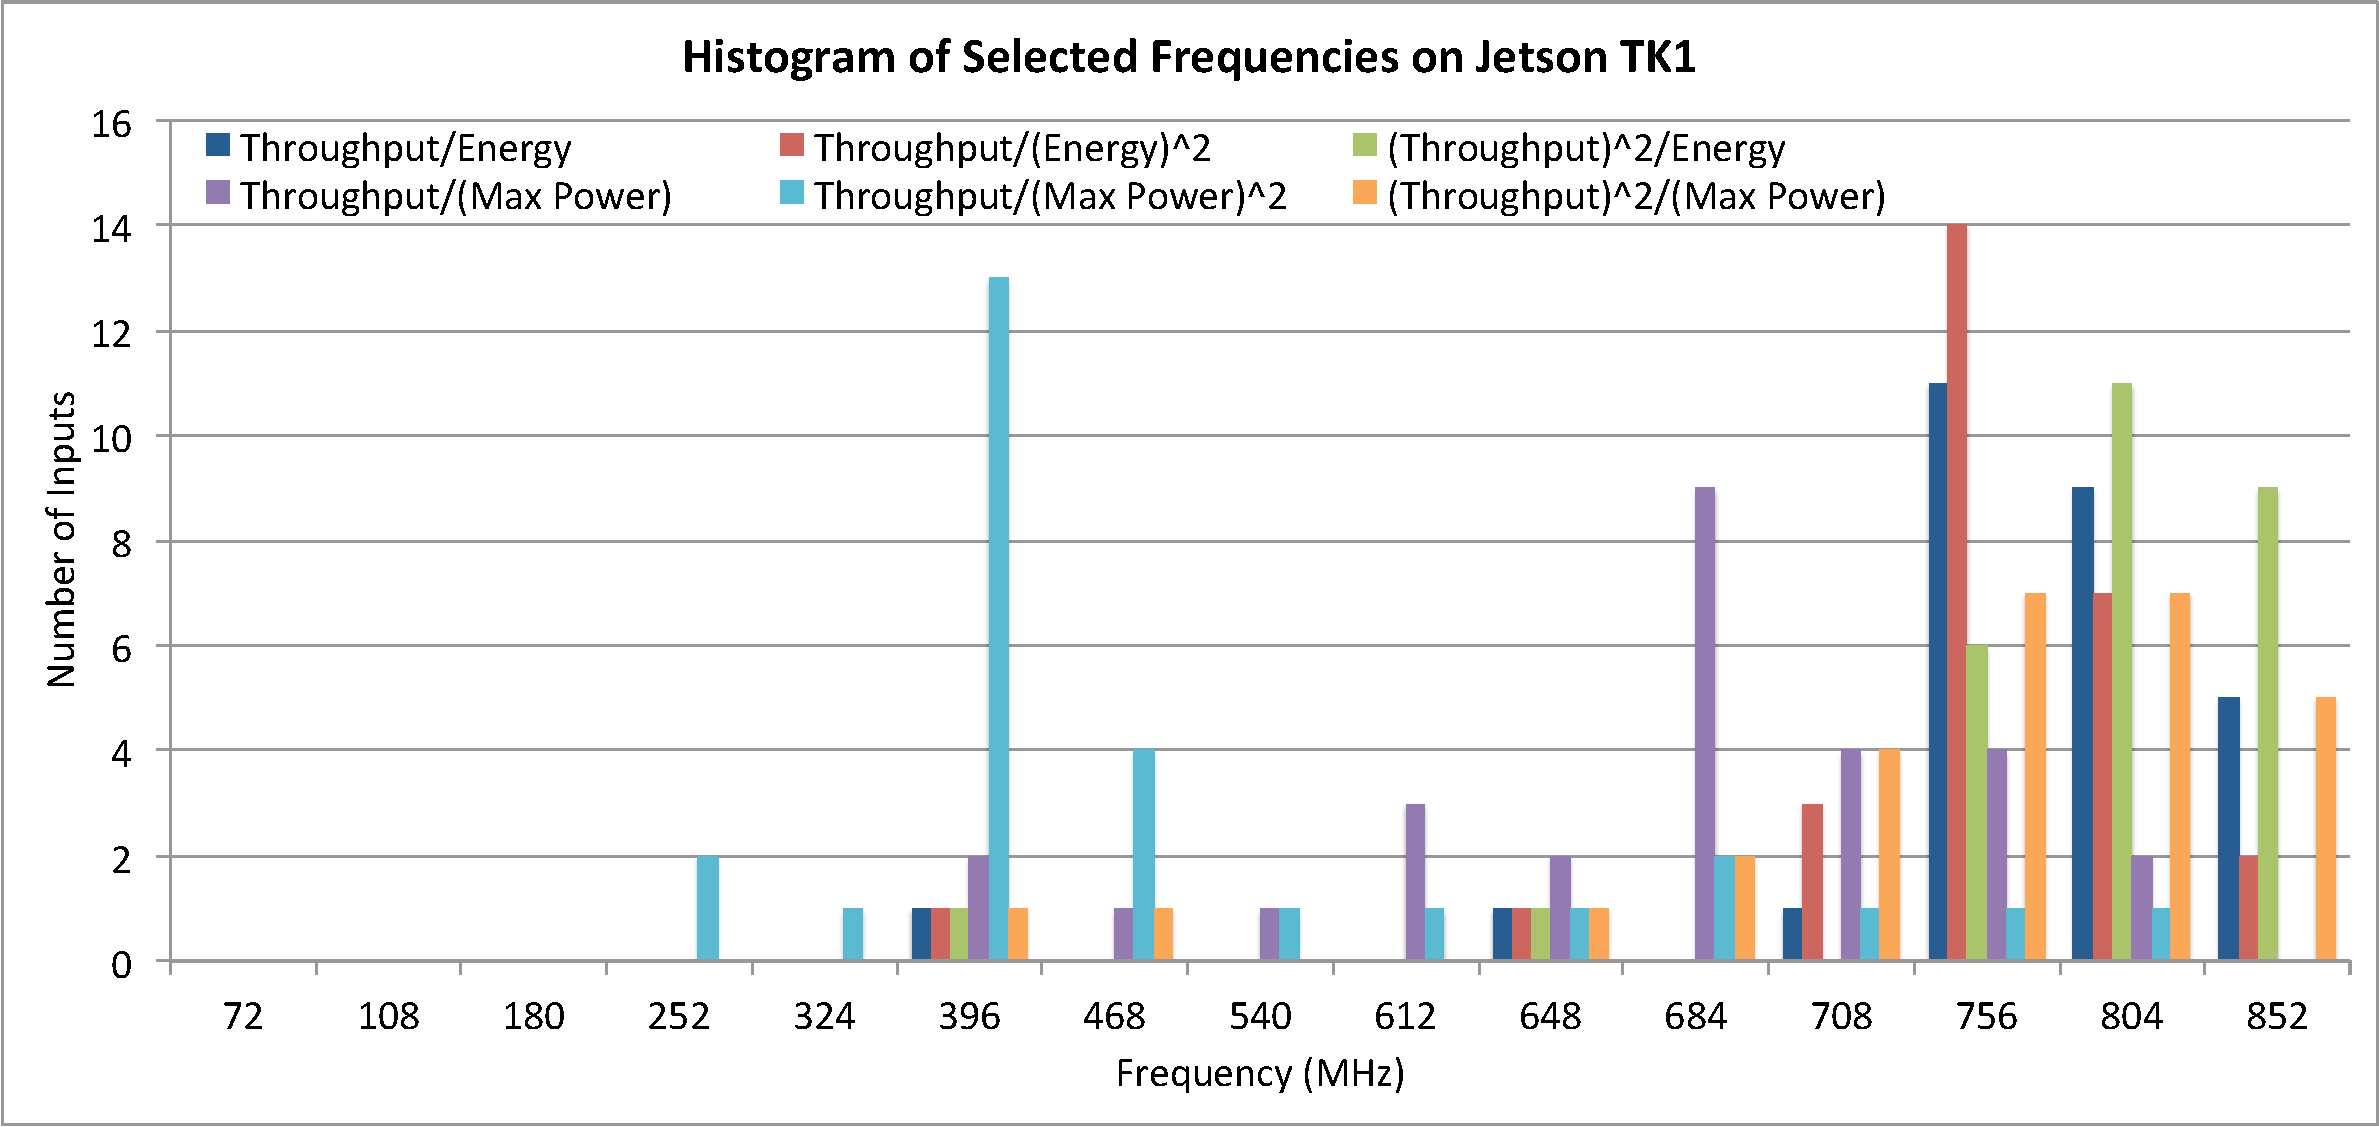
\includegraphics[scale=0.4]{figs/histo_tk1.pdf}
   \caption{Frequencies selected on the Jetson TK1 for various optimization objectives}
   \label{fig:histo-tk1}
\end{figure*}

\begin{figure*}[tb]
   \centering
   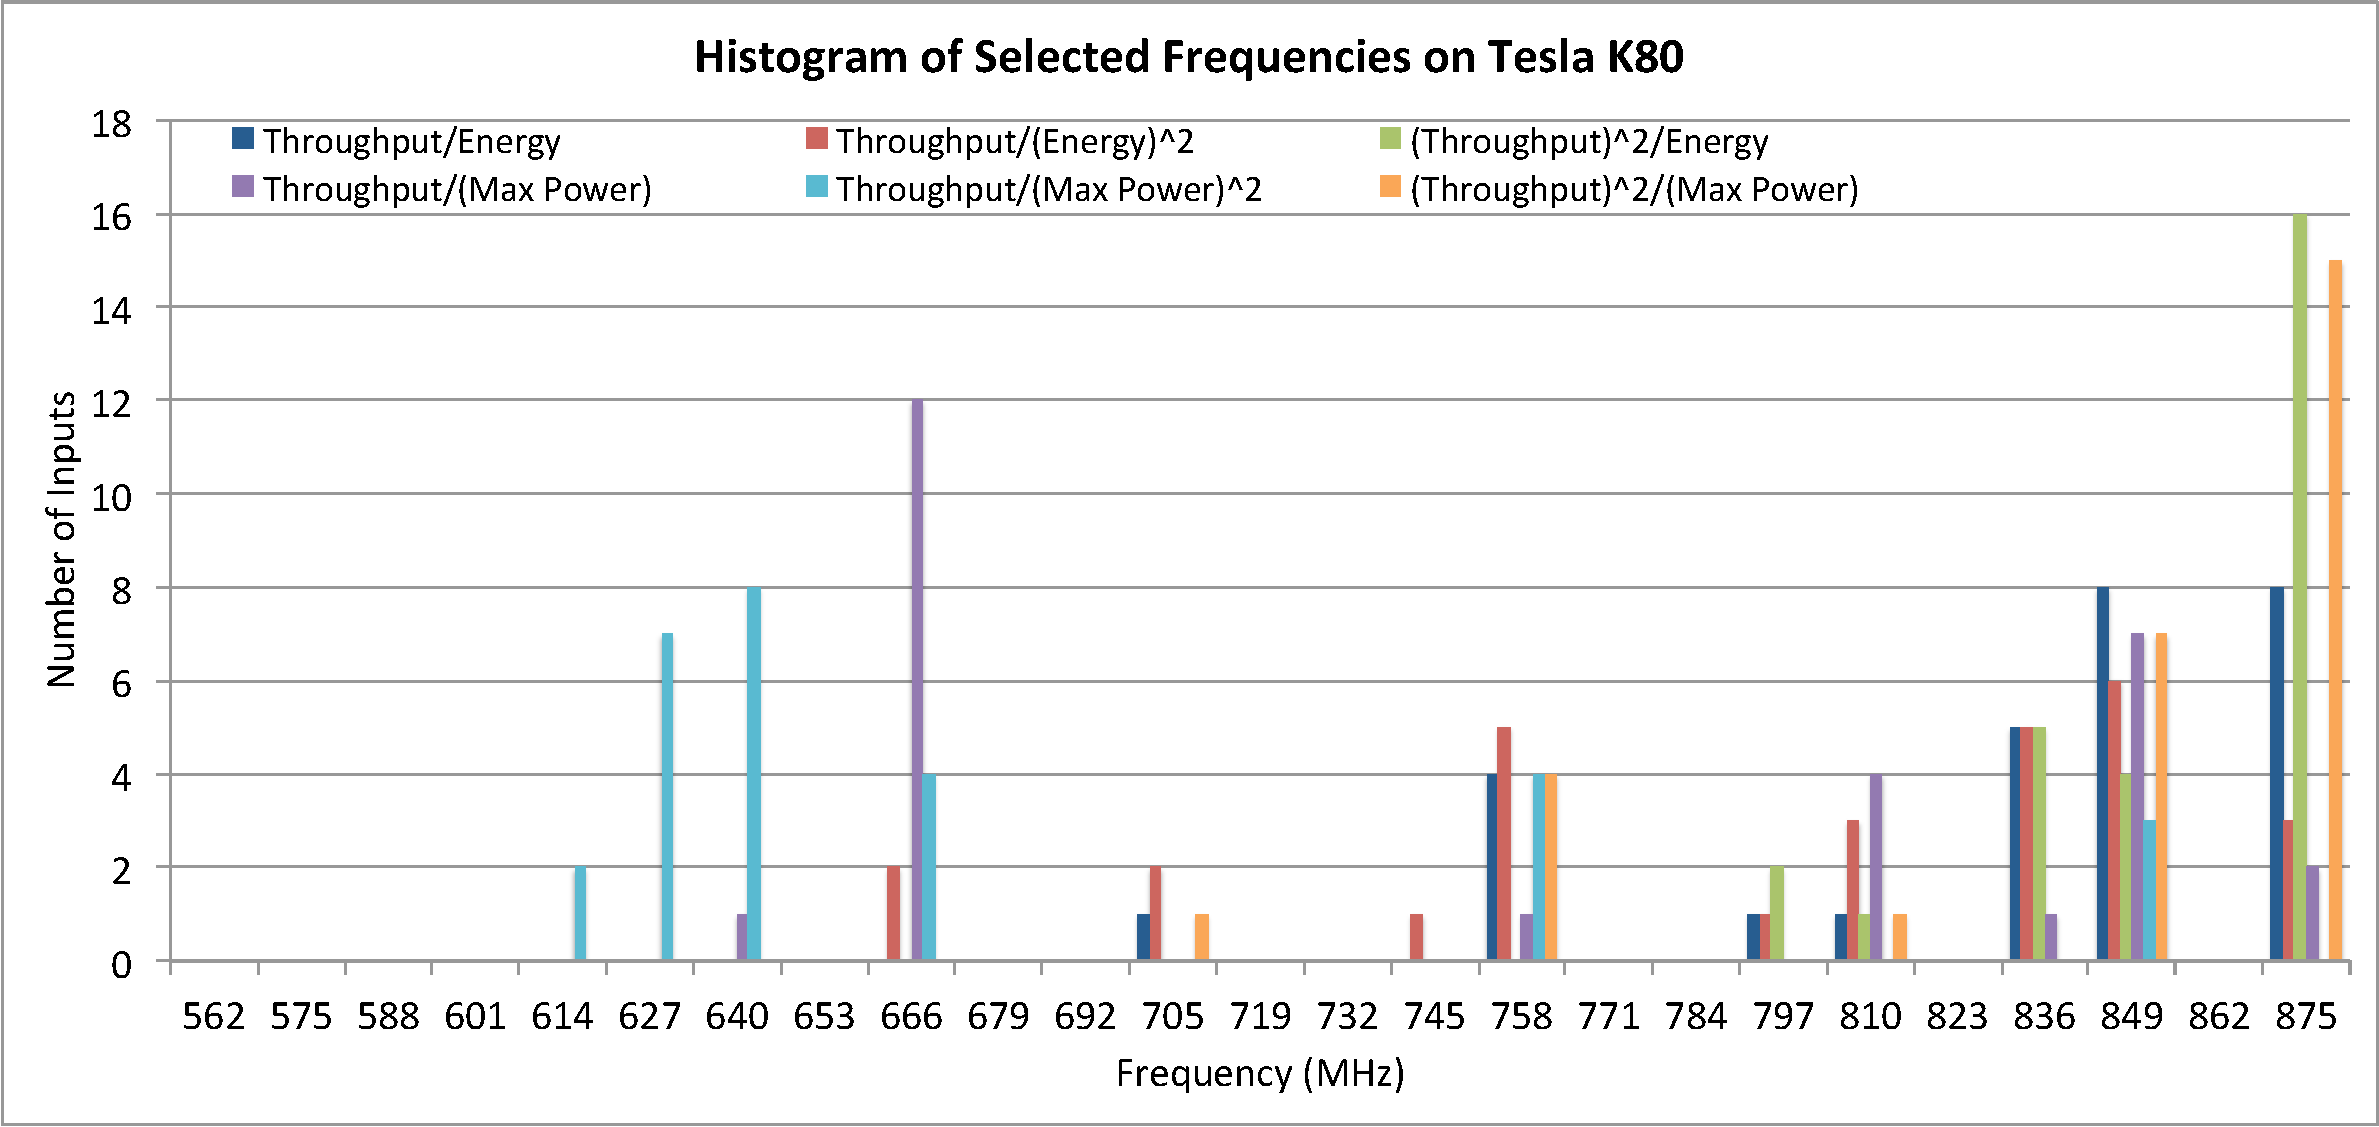
\includegraphics[scale=0.4]{figs/histo_k80.pdf}
   \caption{Frequencies selected on the Tesla K80 for various optimization objectives}
   \label{fig:histo-k80}
\end{figure*}




\setlength\tabcolsep{0 pt}
\begin{figure*}[tb]
\centering
\begin{tabular}{c  c}
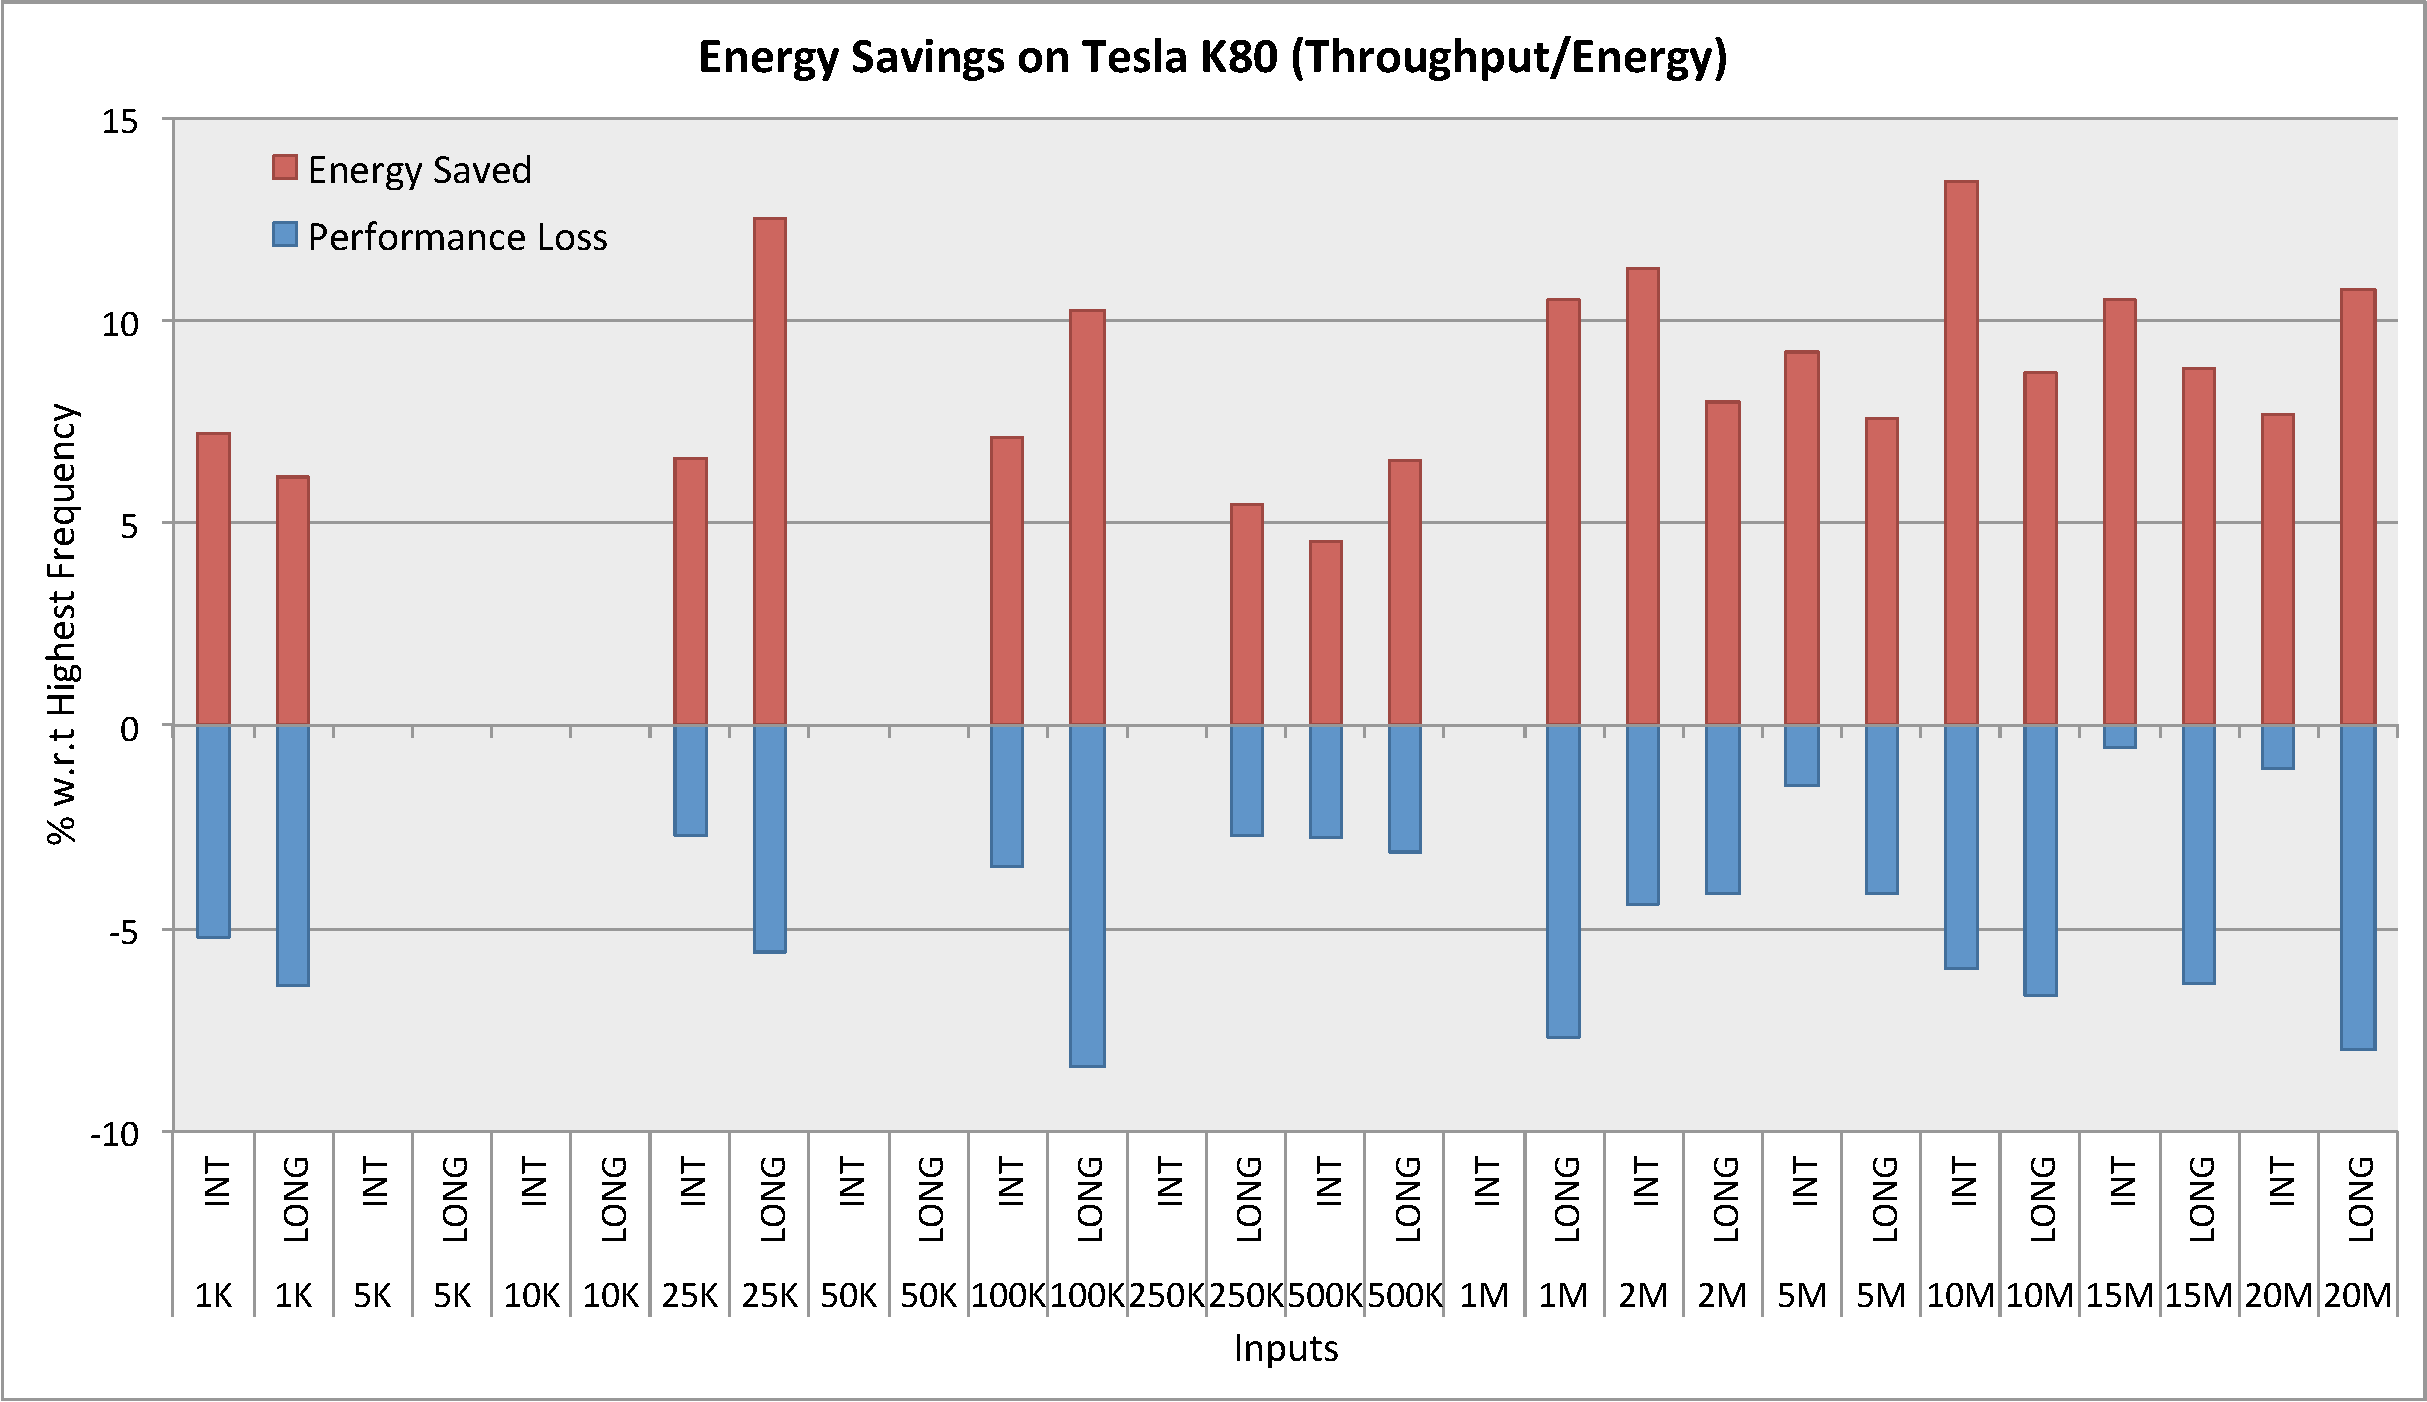
\includegraphics[width=0.5\textwidth]{figs/energy_k80.pdf} &
%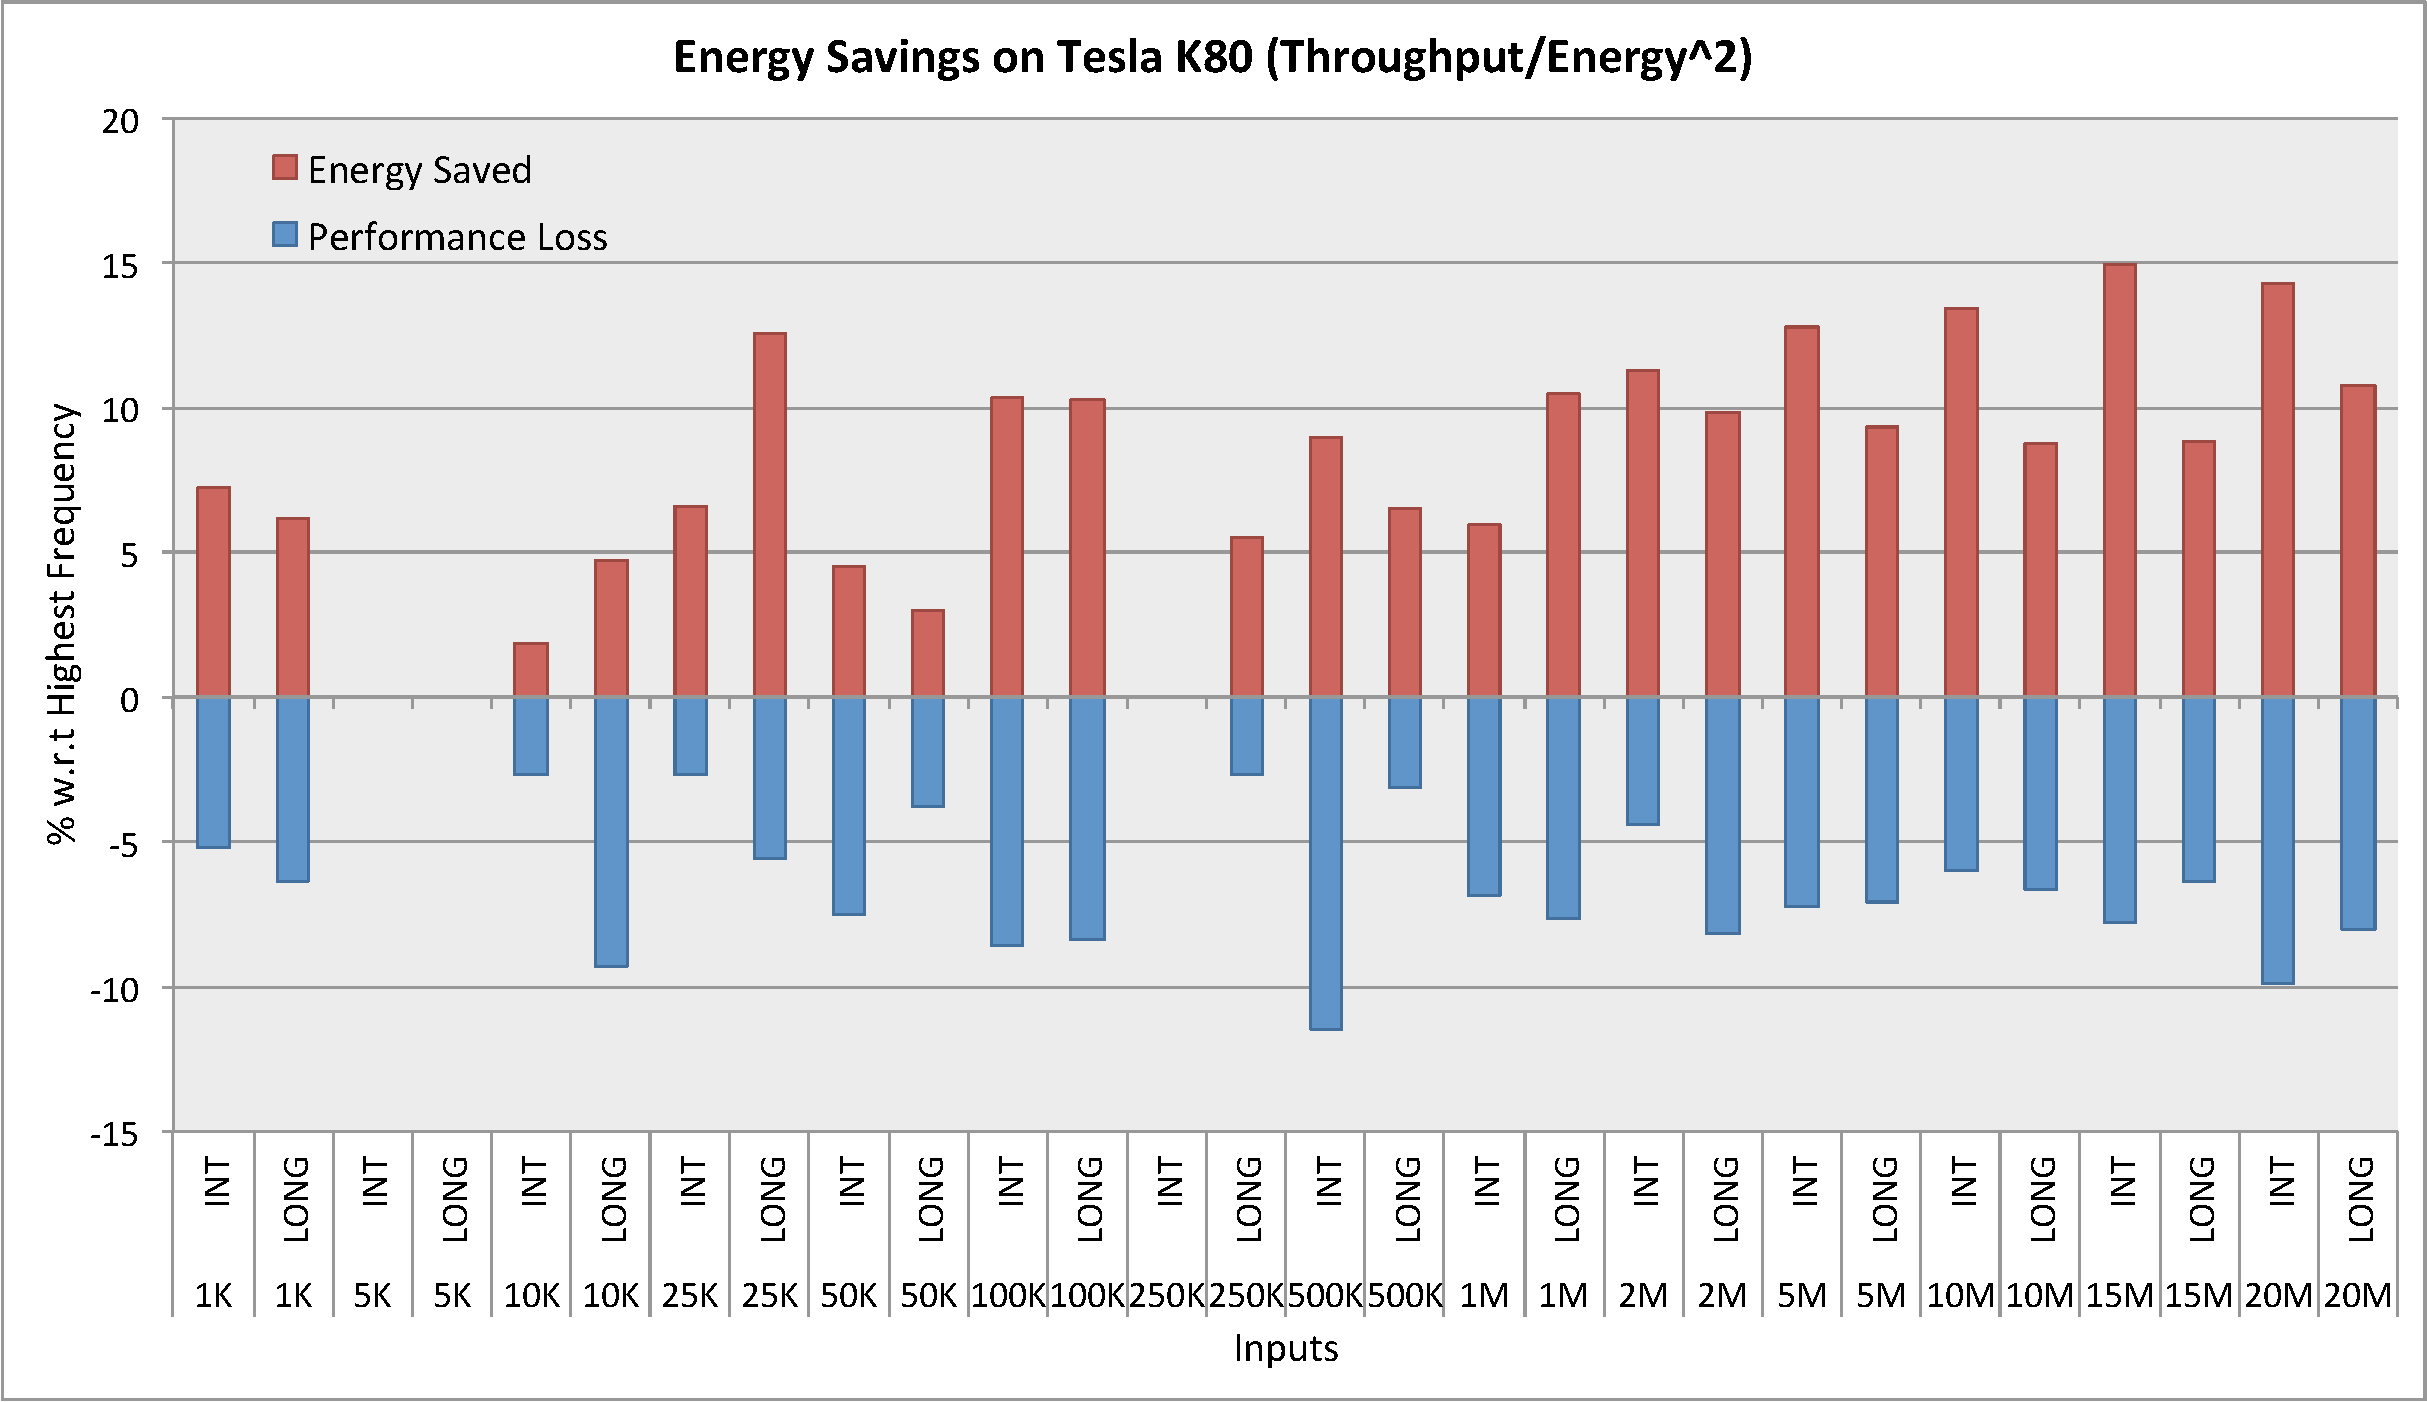
\includegraphics[width=0.4\textwidth]{figs/energy2_k80.pdf} &
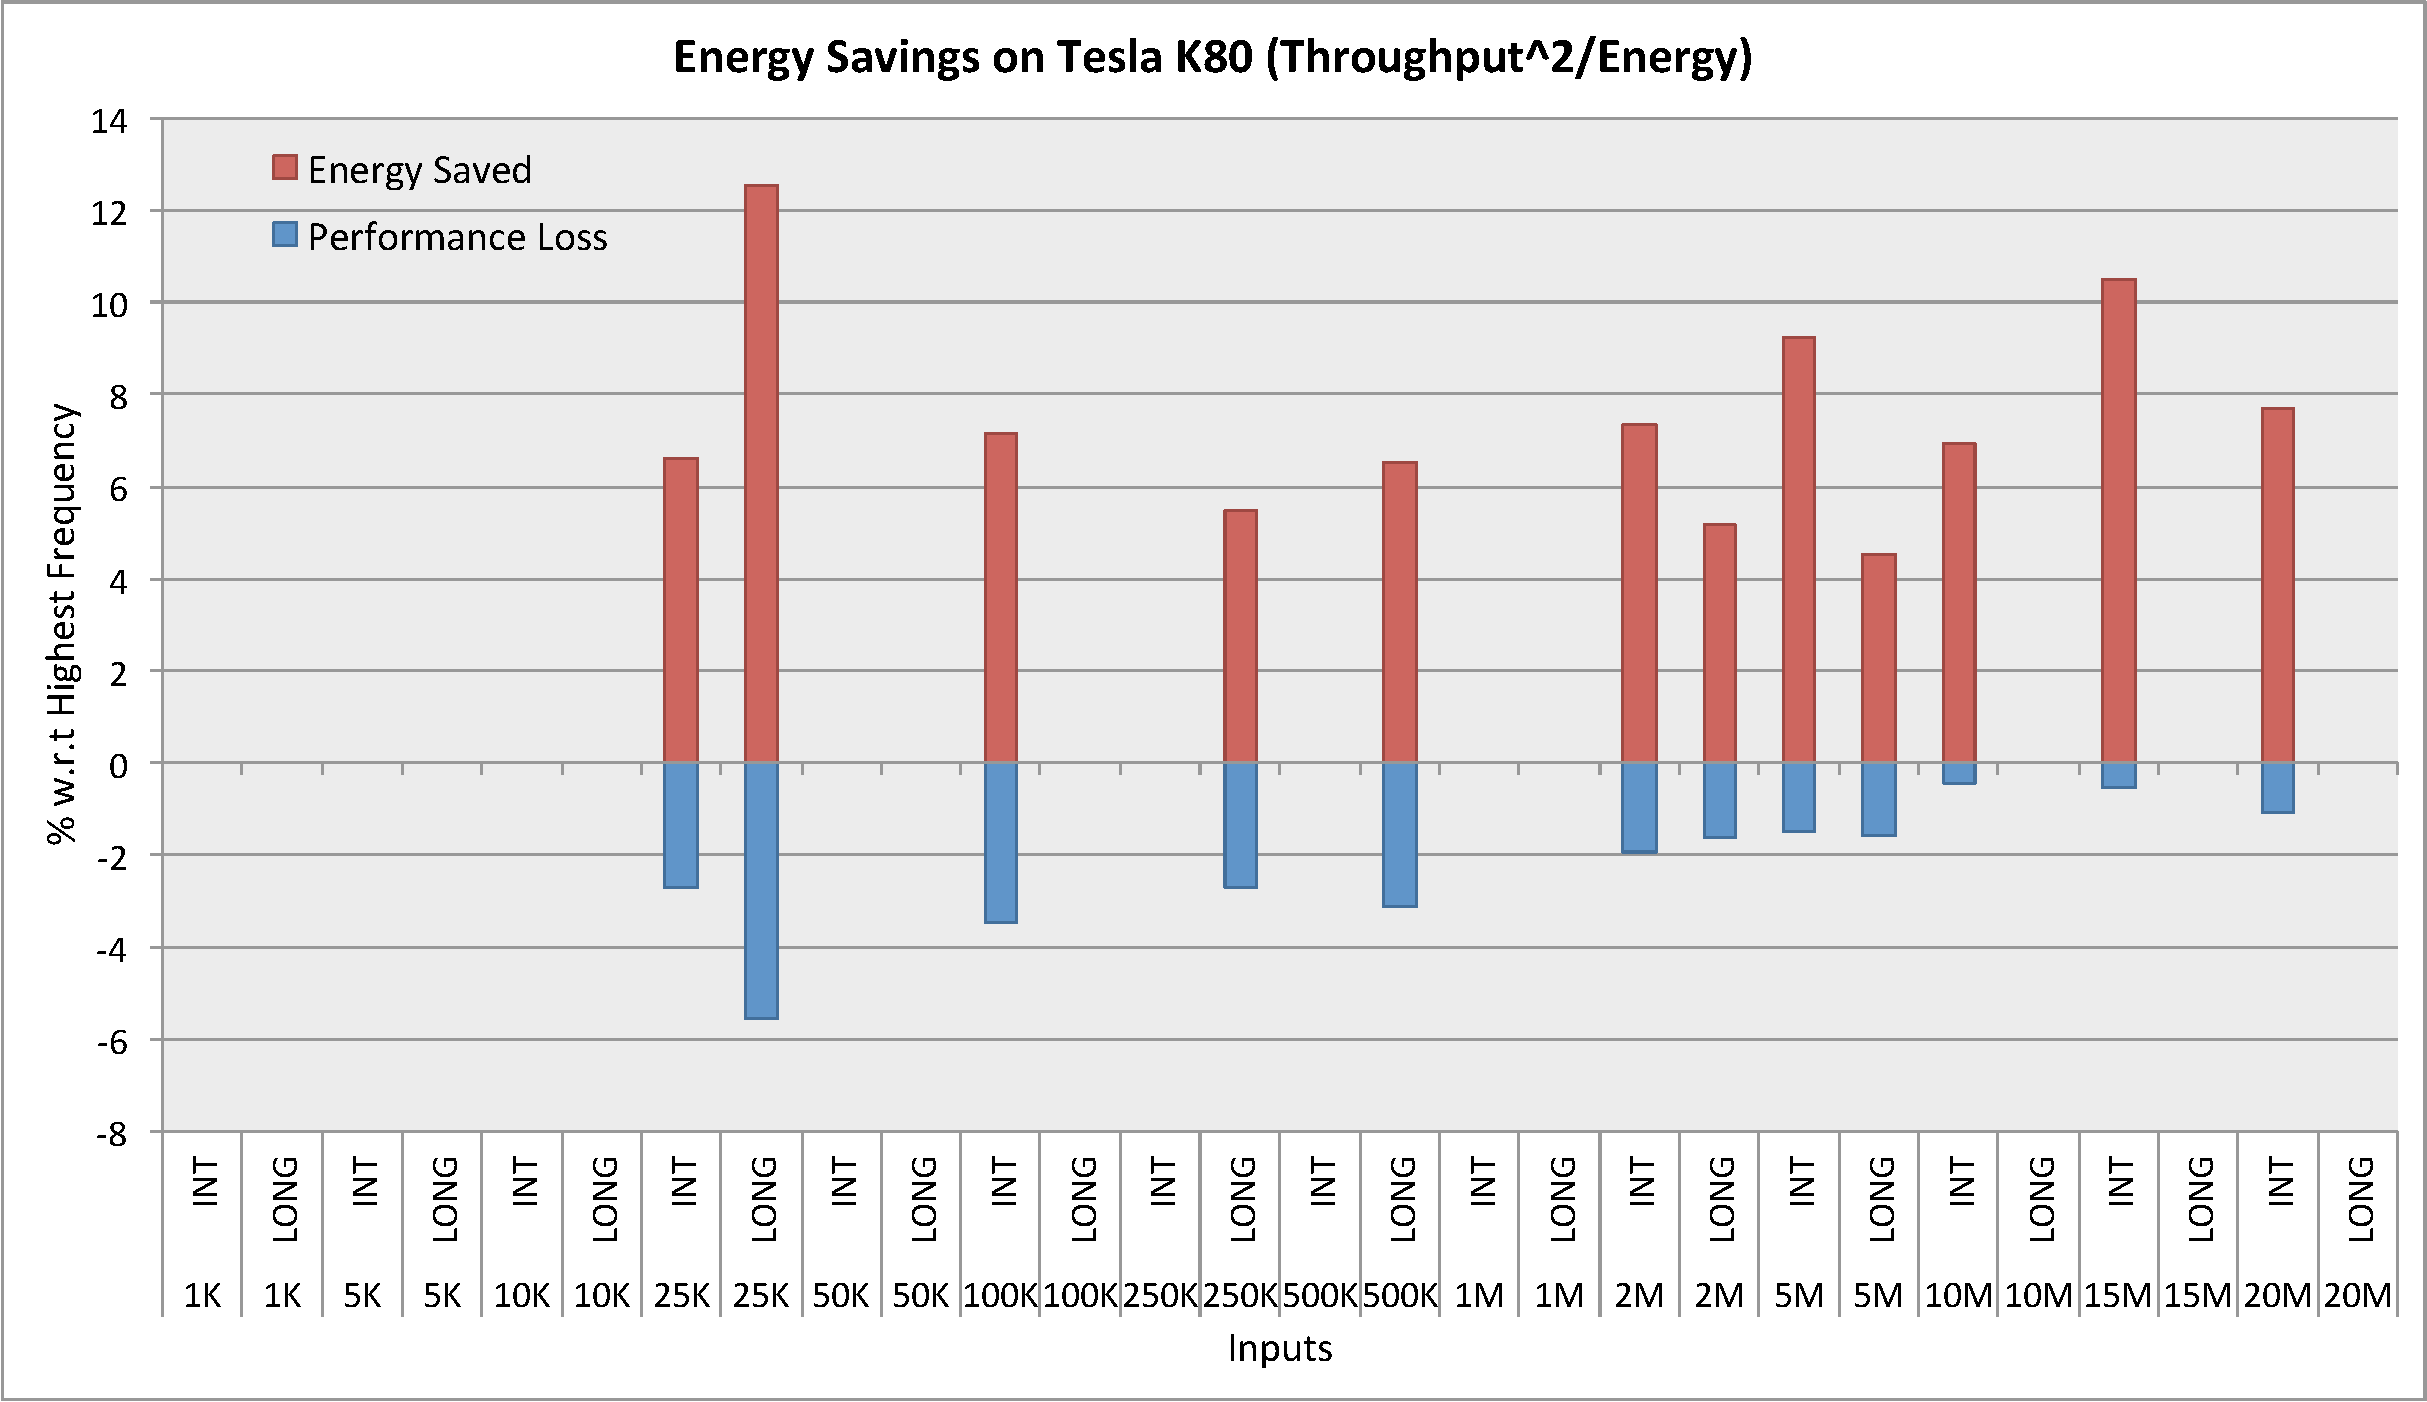
\includegraphics[width=0.5\textwidth]{figs/energy_tp_k80.pdf} \\
%
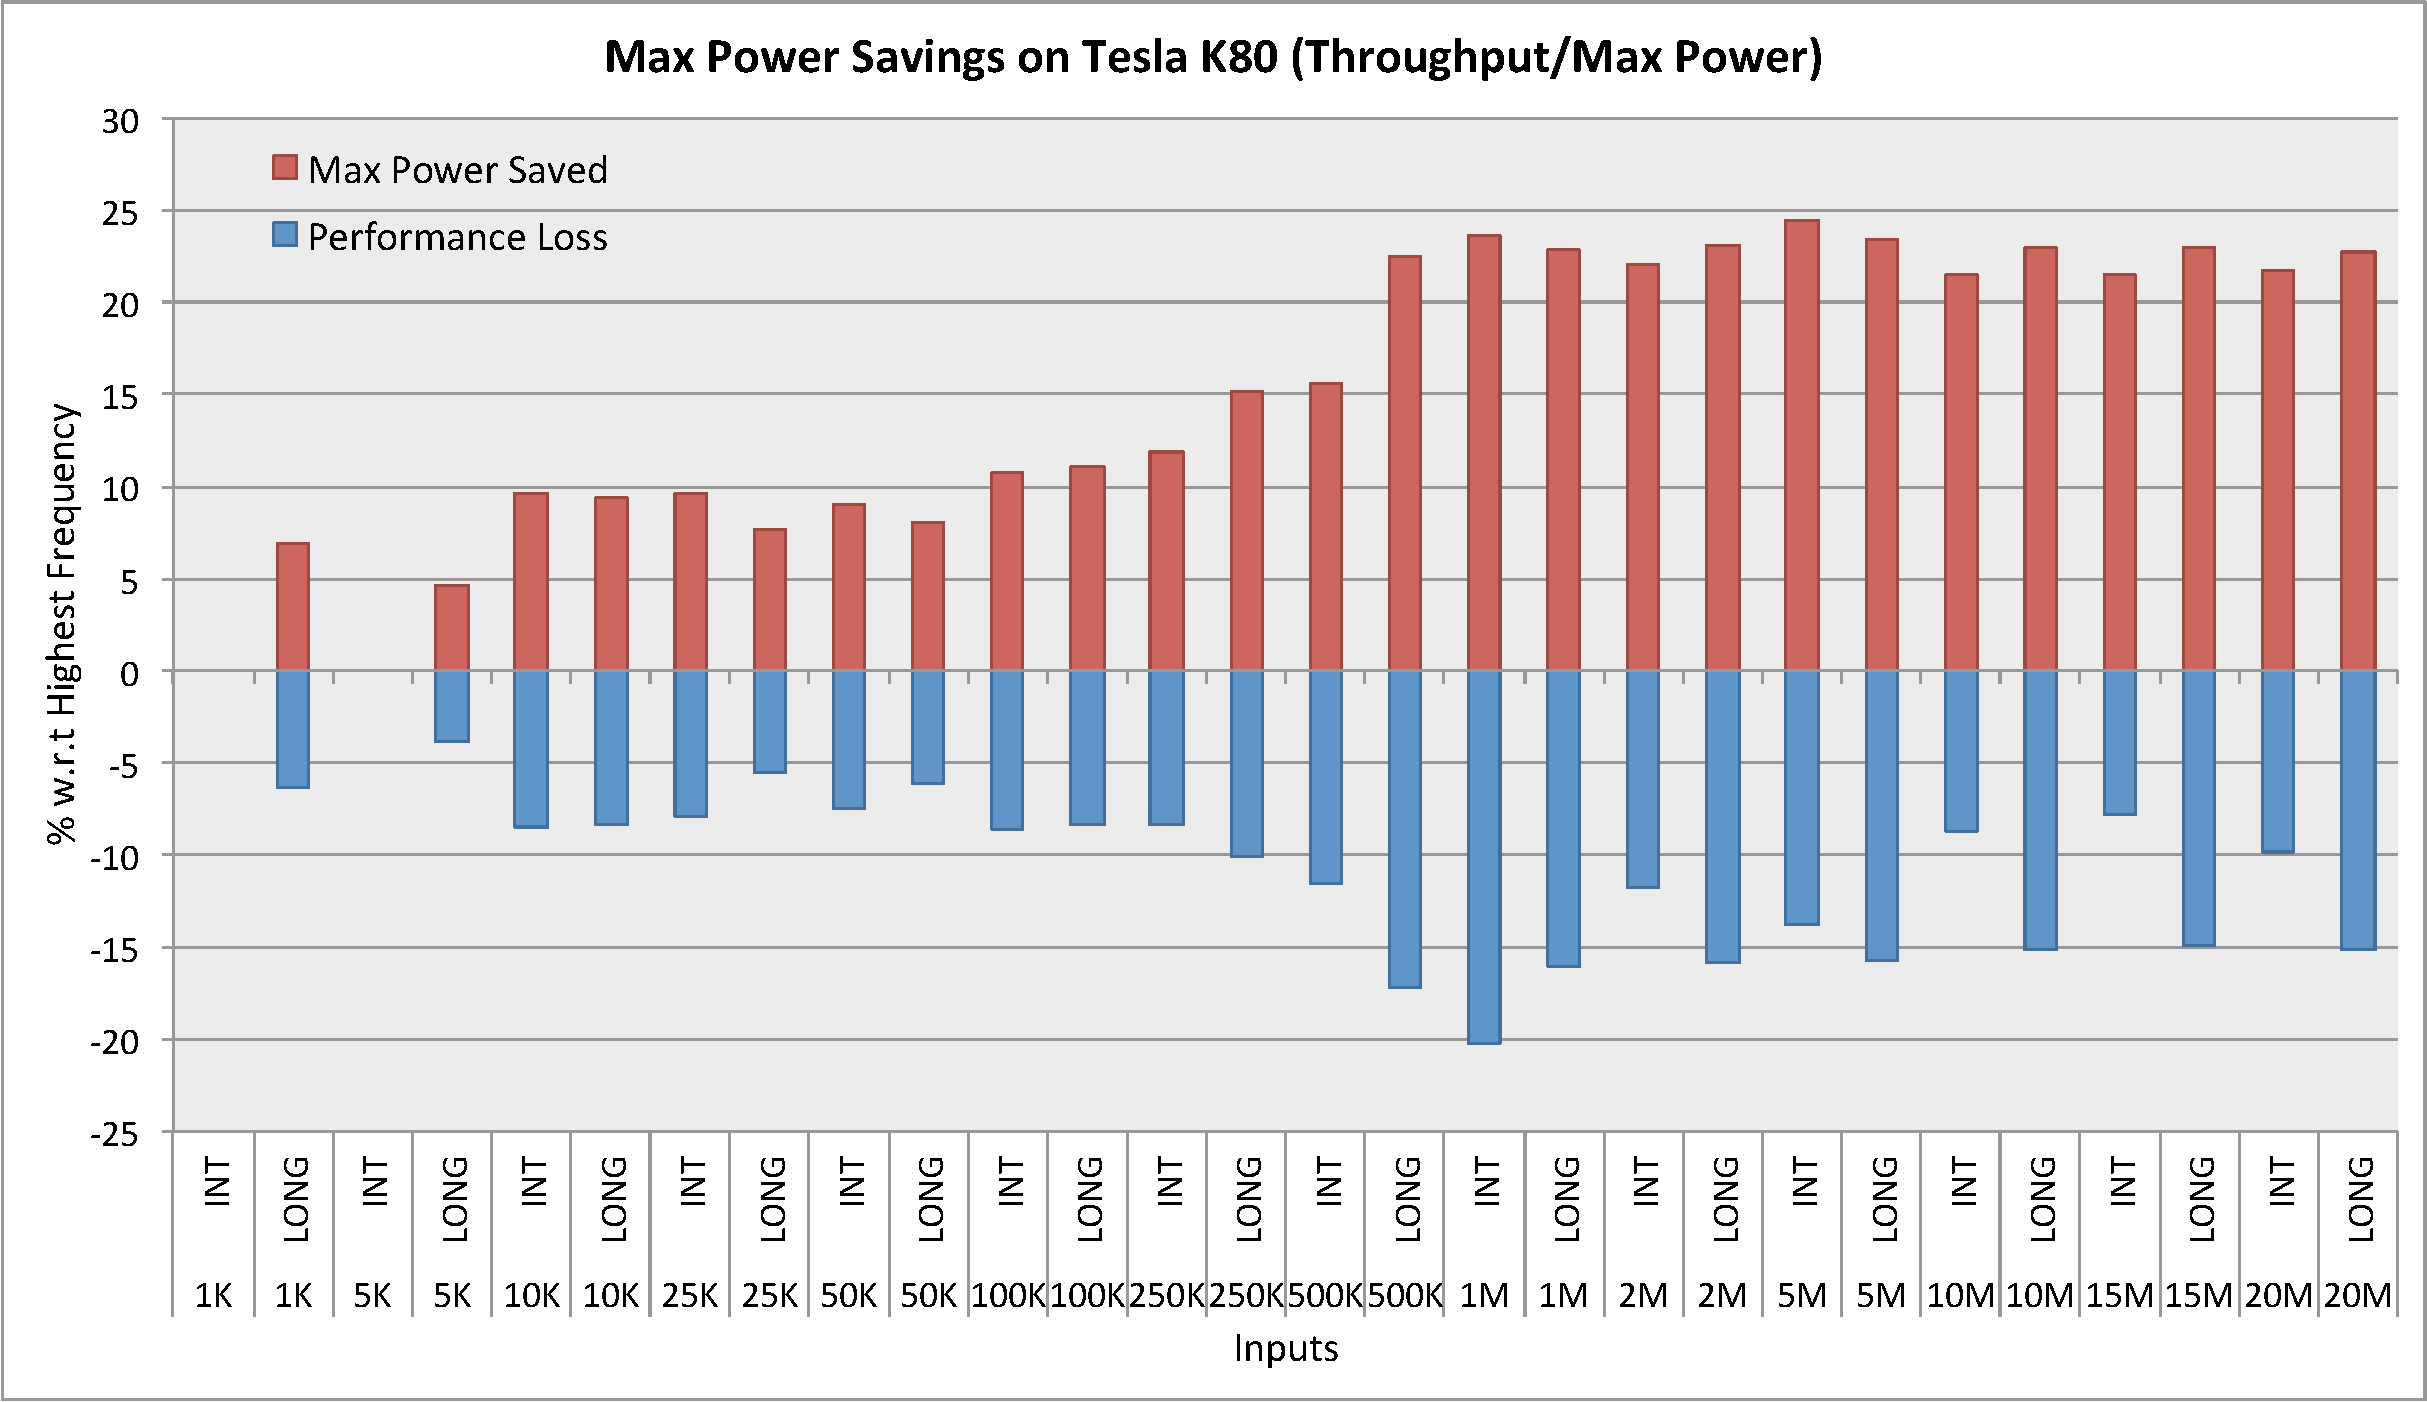
\includegraphics[width=0.5\textwidth]{figs/max_power_k80.pdf} &
%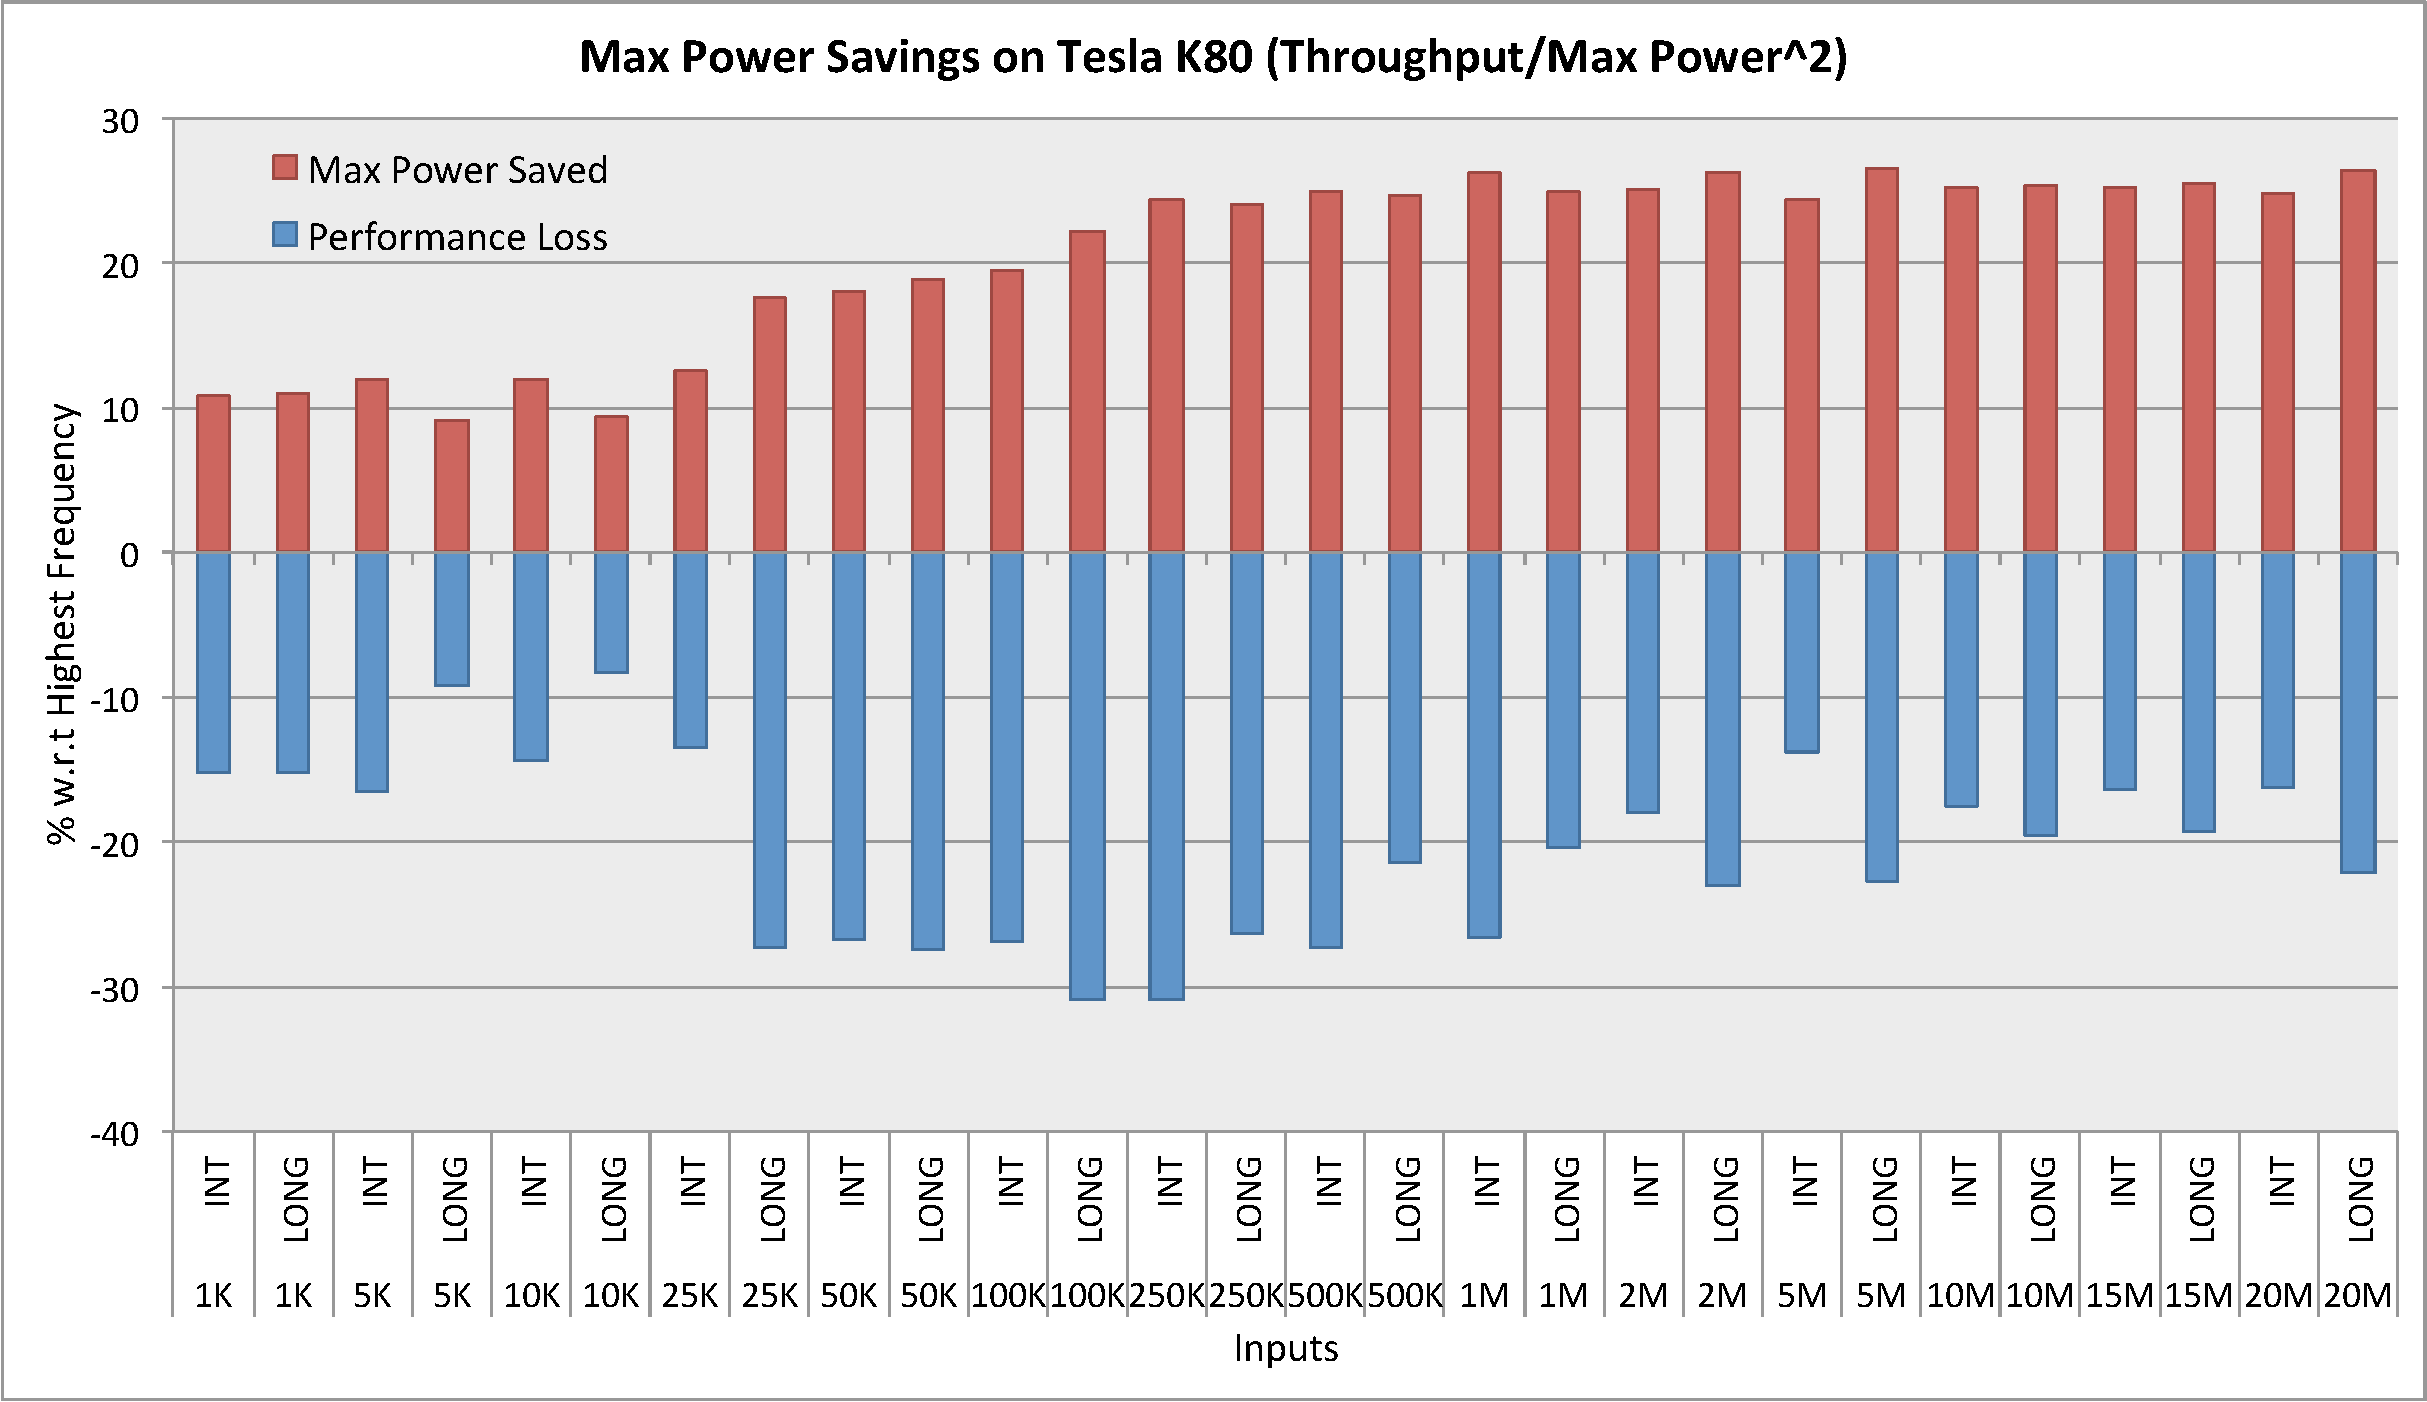
\includegraphics[width=0.4\textwidth]{figs/max_power2_k80.pdf} &
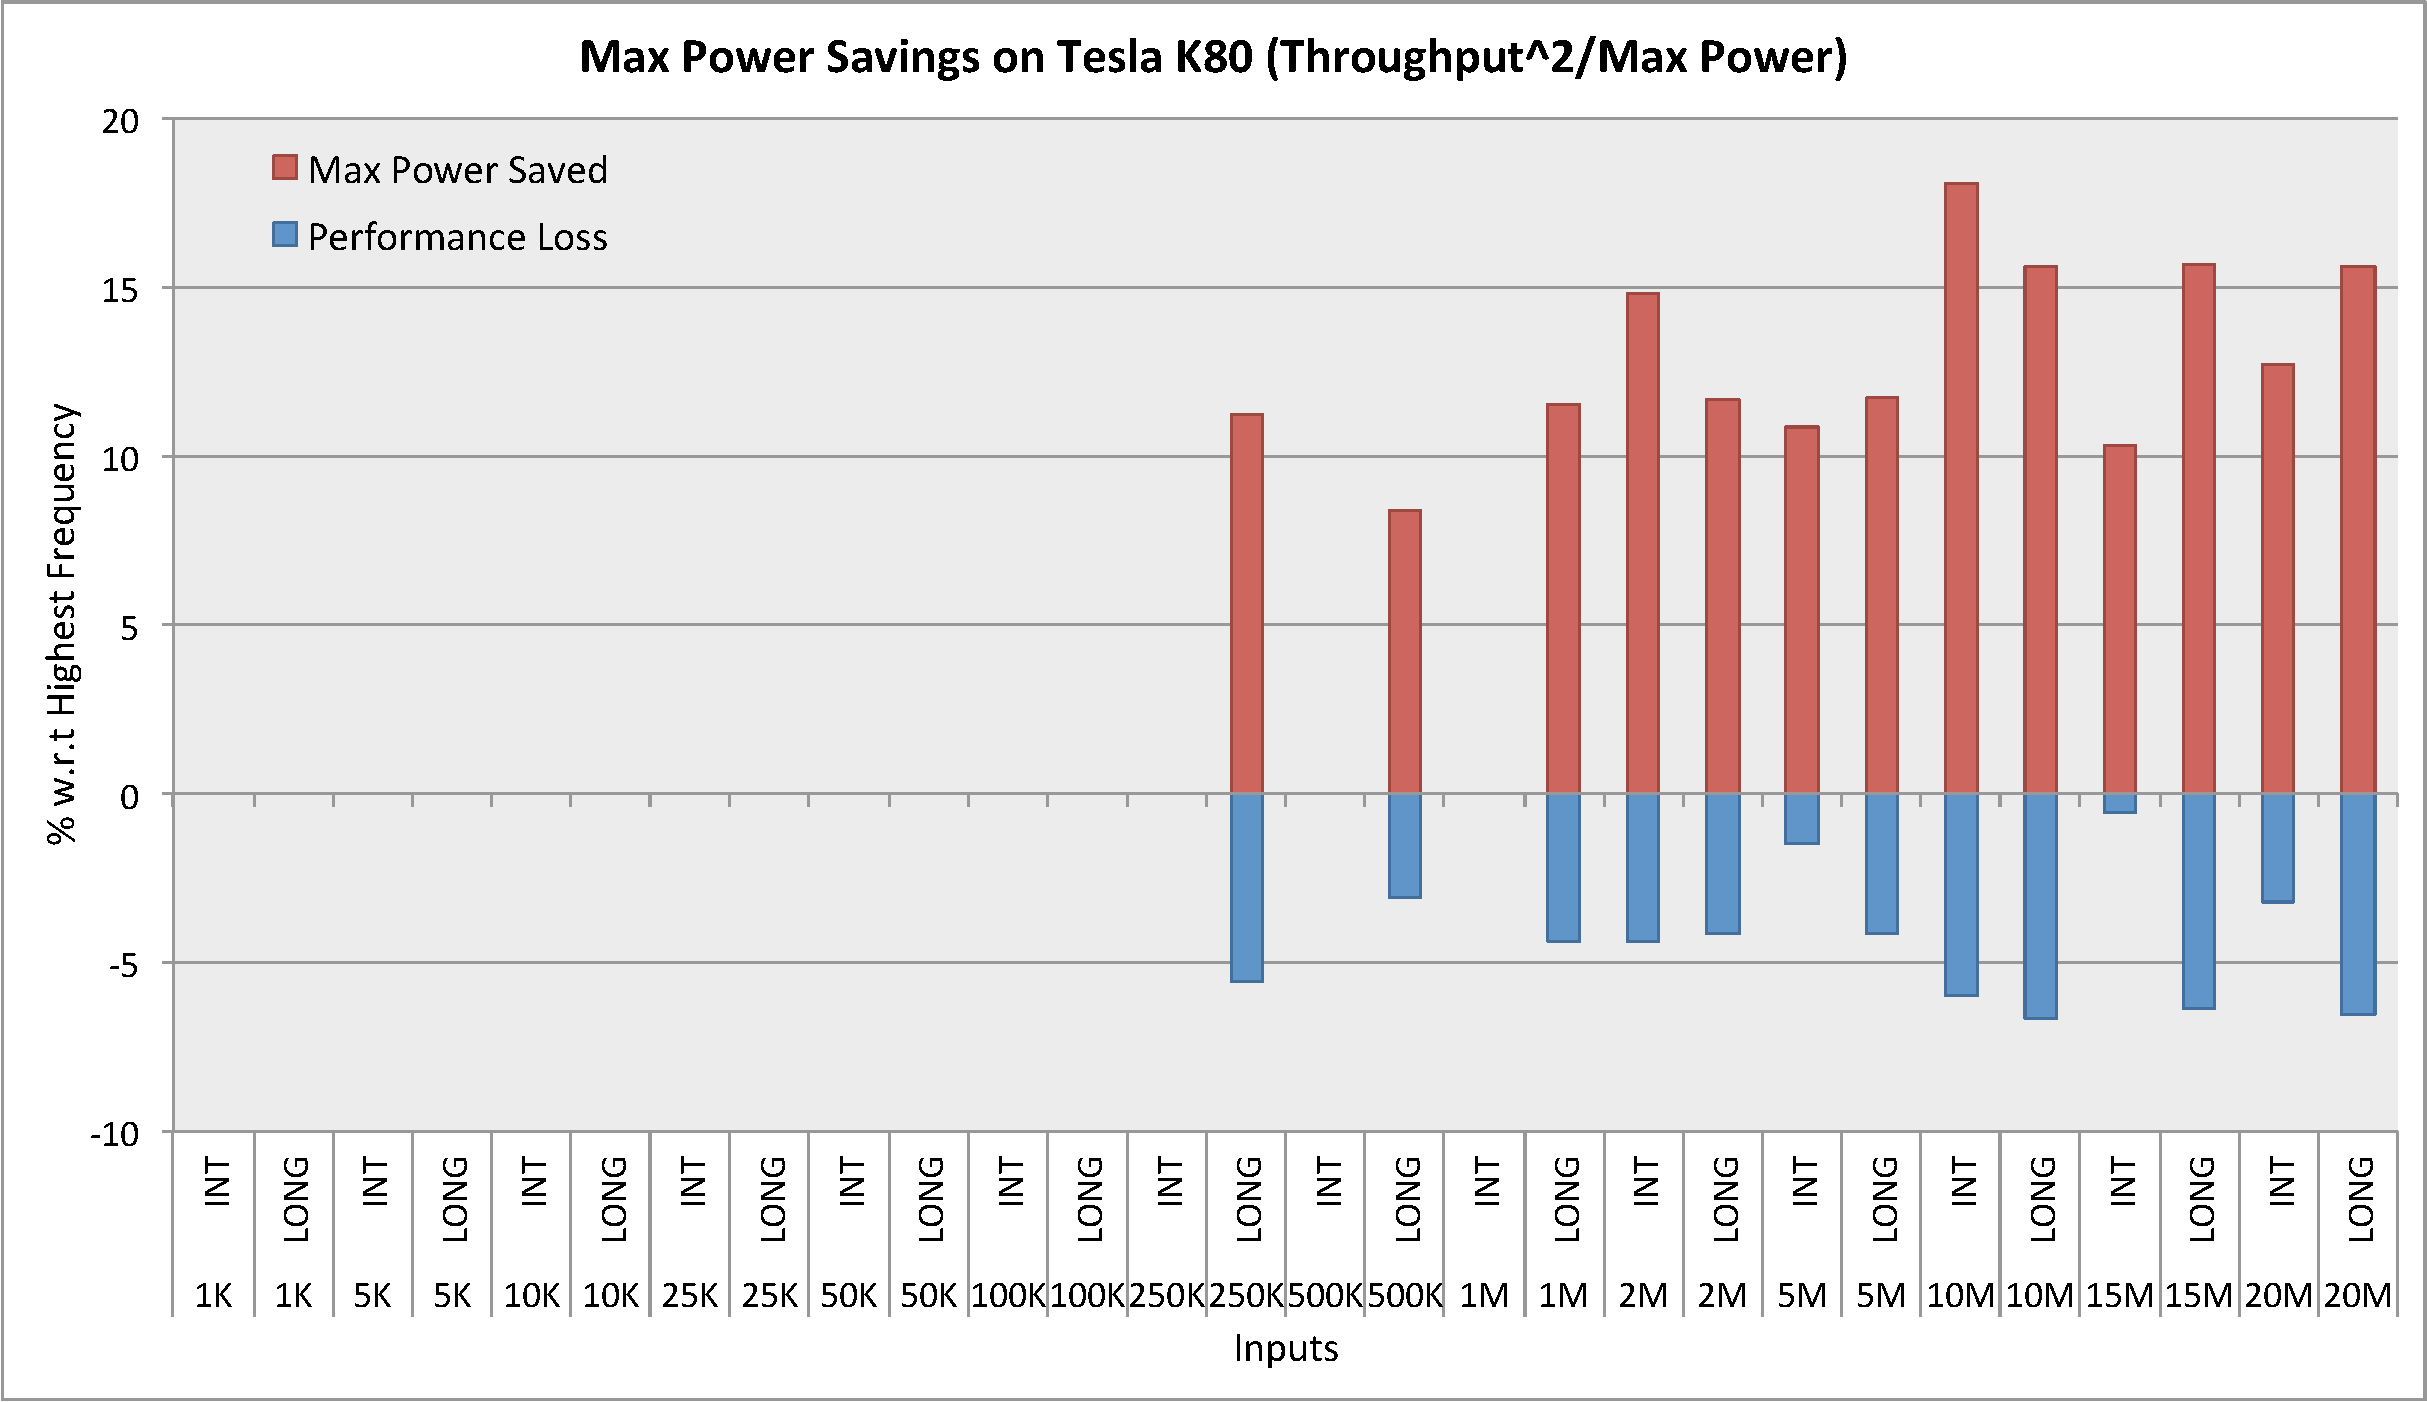
\includegraphics[width=0.5\textwidth]{figs/max_power_tp_k80.pdf} \\

\end{tabular}





\caption{ - }
\label{fig:objective_func}

\end{figure*}
